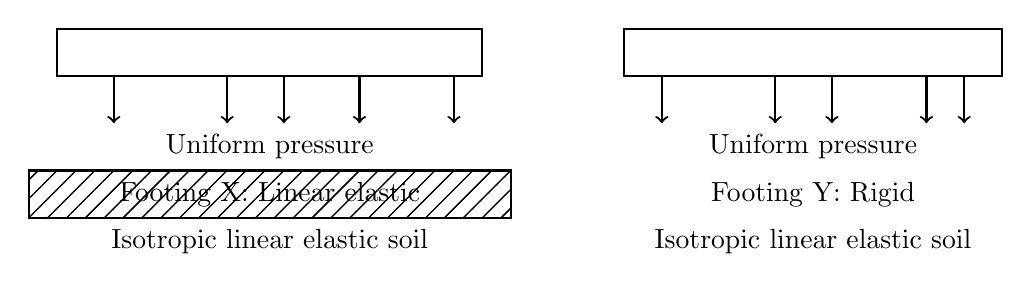
\begin{tikzpicture}[scale=1.2] % Increase scale for larger figure
    % Footing X (Linear Elastic)
    \draw[thick] (0,0) rectangle (4.5,0.5); % Draw footing X
    \foreach \x in {0.6, 1.8, 2.4, 3.2, 4.2} {
        \draw[->, thick] (\x,0) -- (\x,-0.5); % Draw arrows for uniform pressure
    }
    \node at (2.25, -0.75) {Uniform pressure}; % Label for pressure

    % Soil under Footing X
   \begin{scope}
    % Clip to the rectangle
    \clip (-0.3,-1.5) rectangle (4.8,-1);
    % Draw diagonal lines
    \foreach \x in {-5,-4.8,...,10} { % Adjust spacing as needed
        \draw[thin] (\x,-2) -- (\x+2,0); % Adjust angle and spacing
    }
\end{scope}

% Outline the rectangle
\draw[thick] (-0.3,-1.5) rectangle (4.8,-1);
    \node at (2.25, -1.25) {Footing X: Linear elastic}; % Place text inside soil rectangle

    % Gap between Footing X and Footing Y
    \node at (5.5, -0.25) {};

    % Footing Y (Rigid)
    \draw[thick] (6,0) rectangle (10,0.5); % Draw footing Y
    \foreach \x in {6.4, 7.6, 8.2, 9.2, 9.6} {
        \draw[->, thick] (\x,0) -- (\x,-0.5); % Draw arrows for uniform pressure
    }
    \node at (8.0, -0.75) {Uniform pressure}; % Label for pressure

    % Soil under Footing Y
   \begin{scope}
    % Clip to the rectangle
    \clip (-0.3,-1.5) rectangle (4.8,-1);
    % Draw diagonal lines
    \foreach \x in {-5,-4.8,...,10} { % Adjust spacing as needed
        \draw[thin] (\x,-2) -- (\x+2,0); % Adjust angle and spacing
    }
\end{scope}

% Outline the rectangle
\draw[thick] (-0.3,-1.5) rectangle (4.8,-1);    \node at (8.0, -1.25) {Footing Y: Rigid}; % Place text inside soil rectangle

    % Soil Label
    \node at (2.25, -1.75) {Isotropic linear elastic soil}; % Label for soil under footing X
    \node at (8.0, -1.75) {Isotropic linear elastic soil}; % Label for soil under footing Y
\end{tikzpicture}
